\chapter{Antecedentes y estado de la cuestión}
En este capítulo vamos a conocer el estado del arte desde un punto de vista general de las redes de interconexión y, dentro de todos los protocolos de transportes que existen y son usados en estas, vamos a centrarnos en el protocolo RDMA (Remote Direct Memory Access) que nos permite transferir datos de forma más rápida a los protocolos tradicionales como TCP/IP. Una vez desarrollados ambos apartados, vamos a conocer también el entorno que utilizaremos para la simulación del tráfico empleando el mismo escenario y variando entre los dos protocolos de transporte que hemos nombrado y a partir de los cuales obtendremos unos datos que nos servirán para realizar una comparativa del rendimiento de ambos protocolos.

\section{Redes de interconexión}
Las arquitecturas de computación de alto rendimiento utilizan redes de interconexión como base de comunicación entre los núcleos del procesador, los módulos de memoria y los dispositivos de E/S. En su forma más general, las redes de interconexión son un componente central de todos los sistemas informáticos y de comunicación, desde las interconexiones internas de las arquitecturas integradas a nivel de chip hasta los sistemas a escala geográfica, como las redes WAN e Internet. \\

El objetivo de todas las redes de interconexión es transferir información desde cualquier nodo origen a cualquier nodo destino que se desee con la menor latencia posible y permitiendo un gran número de transferencias en ejecución simultánea.\\

Estas redes están compuestas por enlaces y conmutadores, que ayudan a enviar la información entre ambos nodos. Una red esta especificada por su topología, algoritmo de enrutamiento, estrategia de conmutación y mecanismo de control de flujo.\cite{Interconnection}\\

En la figura \ref{fig:redinterconexion} podemos ver seis terminales conectados a una red. Si uno de esos terminales quiere comunicarse con otro de los terminales, envía el mensaje del terminal origen con los datos a través de la red y esta entrega el mensaje al terminal destino.

\begin{figure}[H]
	\centering
	\includegraphics[width=0.5\textwidth]{"/home/vr4/Escritorio/Notas TFG/Imagenes/Red_Interconexión"}
	\caption{Red de Interconexión}
	\label{fig:redinterconexion}
\end{figure}

\subsection{Topología}\label{topology}
Las redes de interconexión están compuestas por elementos de conmutación. La topología de la red se refiere a la disposición estática de los enlaces y los nodos de una red de interconexión: los caminos por los que viajan los paquetes. Esta puede representarse mediante un grafo G(N,C), donde N es el conjunto de los nodos de la red, y C:$NxN$ es el conjuntos de enlaces que conecta un nodo o switch con sus vecinos.\\

Para comprobar que una topología es eficiente, deben evaluarse diferentes parámetros:
\begin{itemize}
	\item \textbf{Ancho de bisección:} se refiere al mínimo número de enlaces que hay que eliminar para dividir la red en dos partes iguales. Un ancho de bisección alto puede reducir el tiempo de comunicación cuando el movimiento de los datos es crítico, ya que la información puede viajar por caminos alternos y evitar así o reducir la congestión en ciertos nodos. Además, esto también hace que el sistema sea más tolerante ante fallos, ya que un nodo defectuoso no hace inoperable al sistema.
	\item \textbf{Grado:} se llama grado de un nodo al número de enlaces que tiene con otros nodos. Es conveniente que en una red el grado sea igual para todos los nodos, siendo en ese caso \textit{regular}. Además, el grado está relacionado directamente con el coste, ya que indica el número de puertos que necesita.
	\item \textbf{Distancia:} Número mínimo de nodos que hay que atravesar para viajar de un nodo origen a un nodo destino. La distancia crea latencia y reducir la distancia entre los distintos nodos es la única forma de poder minimizarla.
	\item \textbf{Distancia media:} representa la media de las distancias de cada par de nodos de la red.
	\item \textbf{Diámetro:} el diámetro es, para par de nodos, el camino más largo de todos los caminos posibles de la red, es decir, el mayor número de enlaces que hay que recorrer en la red para comunicar dos de los nodos que están en ella. Un menor diámetro indica mayor habilidad de comunicación en la red.
	\item \textbf{Longitud de los enlaces:} determina la velocidad a la que la red puede operar y la potencia disipada en ella.
	\item \textbf{Simetría:} se refiere a que desde cualquier nodo la vista de la red presenta el mismo aspecto. Esto implica que una red simétrica tiene que ser regular.
	\item \textbf{Regularidad:} una red es regular si todos los nodos tienen el mismo grado. Es conveniente de cara a la modularidad y escalabilidad.
	\item \textbf{Conectividad:} mínimo número de enlaces o nodos que hay que eliminar para obtener dos gráficos independientes. Cuanto mayor sea el número de enlaces que hay que eliminar para poder dividir la red en dos, mayor es la tolerancia de fallo.
	\item \textbf{Escalabilidad:} facilidad con la que la red puede expandirse manteniendo sus prestaciones sin aumentar su coste en gran medida.
\end{itemize}


Una vez hemos diferenciado los diferentes parámetros que hay que tener en cuenta para comprobar la eficiencia de una red vamos a diferenciar también los diferentes tipos de redes que hay teniendo en cuenta la forma en que se comunican los diferentes nodos.

\subsubsection{Redes de conexión de medio compartido}
Estas redes están formadas por un único elemento común de interconexión al que se conectan directamente todos los nodos de la red. No son muy utilizadas en computación paralela debido a sus bajas prestaciones. Estas redes se pueden clasificar en:\cite{shareNetworks} 

\paragraph{Redes de área local}
Permiten comunicar equipos distanciados varios metros entre sí.

\begin{figure}[H]
	\centering
	\includegraphics[width=0.5\linewidth]{"../../Notas TFG/Imagenes/Red_Area_Lpcal"}
	\caption{Red de área local}
	\label{fig:redarealocal}
\end{figure}

\subparagraph{Bus de contención (CSMA/CD)}
Acceso al bus compartido mediante competencia entre los dispositivos y resolución de colisiones. Es un algoritmo no determinista, por lo que no se puede garantizar el tiempo de espera de un dispositivo hasta obtener acceso al bus.

\subparagraph{Token Bus}
Dispositivos conectados en modo broadcast al bus. Se utiliza un token que circula entre los dispositivos en orden para habilitar el uso del bus.

\begin{figure}[H]
	\centering
	\includegraphics[width=0.4\linewidth]{"../../Notas TFG/Imagenes/Token_Bus"}
	\caption{Topología token bus}
	\label{fig:tokenbus}
\end{figure}

\subparagraph{Token Ring}
Dispositivos conectados en anillo físico. Uso de un token que circula entre los dispositivos para dar acceso al bus.

\begin{figure}[H]
	\centering
	\includegraphics[width=0.5\linewidth]{"../../Notas TFG/Imagenes/Token_Ring"}
	\caption{Topología token ring}
	\label{fig:tokenring}
\end{figure}

\subsubsection{Redes de conexión directas o estáticas}
Una red directa está formada por un conjunto de nodos que están conectados mediante enlaces point-to-point a un pequeño subconjunto de nodos. Cada uno de los nodos que componen la red realiza tanto el enrutamiento como la computación.\\
Entre las propiedades de las redes directas tenemos las especificadas en la sección \ref{topology} y, además, la propiedad ortogonal, es decir que todos los nodos y enlaces que componen la red pueden disponerse en \textit{n} dimensiones, de manera que cada enlace está situado exactamente en una dimensión. En las redes directas, los caminos para la transmisión de mensajes se seleccionan mediante algoritmos de encaminamiento. mientras que los mecanismos de conmutación determinan cómo se conectan las entradas a las salidas en un nodo.\\

Dentro de las redes de conexión directas podemos distinguir distintos tipo dependiendo de como se distribuyan y se conecten los nodos entre sí:

\paragraph{Estrella} 
En esta red existe un nodo central que se conecta con todos los demás nodos de la red. El inconveniente de esta red es que, cuando el número de nodos que se conectan al nodo central es alto, esta topología ya no es práctica ya que, al tener que atravesar todos los mensajes el nodo central, se sobrecarga la red.

\begin{figure}[!h]
	\centering
	\includegraphics[width=0.4\textwidth]{"/home/vr4/Escritorio/Notas TFG/Imagenes/Red_Estrella"}
	\caption{Topología estrella}
	\label{fig:redestrella}
\end{figure}

\paragraph{Anillo}
Al igual que la topología estrella, es una de las formas de conexión más simples pues se conectan los nodos que situándose todos en una fila, por lo que cada nodo tiene dos nodos vecinos a los que se conecta formando una circunferencia de nodos conectados. Para encaminar un mensaje de un nodo a otro, una vez determinado por  qué enlace debe enviarse, únicamente hay que transmitirlo hasta que llegue al nodo destino. 

\begin{figure}[H]
	\centering
	\includegraphics[width=0.4\textwidth]{"/home/vr4/Escritorio/Notas TFG/Imagenes/Red_Anillo"}
	\caption{Topología anillo}
	\label{fig:redanillo}
\end{figure}

\paragraph{Malla}
Una malla es una topología de red directa que posee n dimensiones en la que cada una de ellas hay k nodos, por ello el número de nodos de la red es $k*n$ y cada uno de estos vértices está conectado a todos aquellos que difieren en una coordenada de él en cualquiera de las dimensiones. Esta topología no es regular, ya que los nodos interiores tienen grado 2n y los nodos exteriores tienen grado n.\\
Una de las características esenciales de la malla es que es infinitamente extensible según k y según n hasta el límite de las interconexiones disponibles; en este sentido, es la más modular de las topologías.

\begin{figure}[H]
	\centering
	\includegraphics[width=0.3\textwidth]{"/home/vr4/Escritorio/Notas TFG/Imagenes/Red_Malla"}
	\caption{Topología Malla}
	\label{fig:redmalla}
\end{figure}

\paragraph{Toro}
Las redes en toro son mallas en que sus filas y columnas tienen conexiones en anillo, lo que contribuye a disminuir su diámetros. Esta modificación convierte a las mallasen estructuras simétricas y además, reduce su diámetro a la mitad. 
\begin{figure}[H]
	\centering
	\includegraphics[width=0.3\linewidth]{"/home/vr4/Escritorio/Notas TFG/Imagenes/Red_toro"}
	\caption{Topología toro}
	\label{fig:redtoro}
\end{figure}


\paragraph{Hipercubo}
Las redes con topología hipercubo están formadas por $2^{n}$ nodos, que forman los vértices de los cuadrados para crear una conexión entre redes. Esta conexión se realiza conectando los nodos que solo difieren en un bit en su representación binaria (como vemos en la figura \ref{fig:redhipercubo}). Un hipercubo es básicamente una red de malla multidimensional con dos nodos en cada dimensión.  

\begin{figure}[H]
	\centering
	\includegraphics[width=0.4\linewidth]{"../../Notas TFG/Imagenes/Red_Hipercubo"}
	\caption{Topología hipercubo}
	\label{fig:redhipercubo}
\end{figure}


\subsubsection{Redes de conexión indirectas o dinámicas}
Estas redes, a diferencia de las redes de conexión directa, no tienen vecinos fijos. La topología de comunicación puede cambiarse dinámicamente en base a las demandas de la aplicación. 

\paragraph{Redes en bus}
Estas redes están compuestas por una serie de líneas de bits a las que se conectan varios recursos (Figura \ref{fig:redenbus}). El inconveniente de un bus es que sólo permite una transferencia al mismo tiempo, por ello, cuando hay varios recursos que tratan de conectarse al bus, se necesita un árbitro que será de ir dando paso, una a una, a las diferentes peticiones. Los buses son una forma barata de comunicación que tienen la ventaja de ser muy fácilmente reconfigurables, pero con la desventaja de un bajo ancho de banda y una gran latencia debida a las continuas esperas de las peticiones.
	
	\begin{figure}[H]
		\centering
		\includegraphics[width=0.4\textwidth]{/home/vr4/Escritorio/Notas TFG/Imagenes/Red_en_bus}
		\caption{Red en bus}
		\label{fig:redenbus}
	\end{figure}

\paragraph{Redes multietapa}	
Estas redes están formadas por múltiples etapas de switches. Se compone de interruptores 'axb', siendo 'a' el número de entradas del switch y 'b' el de salidas, que se conectan mediante un patrón de conexión interetapas (ISC) determinado. La ventaja de estas redes sobre la redes crossbar es el menor número de conmutadores, que varía dependiendo del tipo de red, sin embargo, algunas de ellas son bloqueantes. Entre las redes multietapa tenemos, entre otros, los siguientes tipos:
	

\subparagraph{Redes Omega}
Estas redes están formadas por N etapas siendo N el número de entradas de la red. En este tipo de red es posible llegar a varios destinos a partir de un solo origen, permitiendo realizar difusiones en la red. Por el contrario, estas redes son sensibles a fallos ya que, si un hilo se corta, no serán posibles muchas de las rutas.

\newpage			

			\begin{figure}[H]
				\centering
				\includegraphics[width=0.45\textwidth]{"/home/vr4/Escritorio/Notas TFG/Imagenes/Red_multietapa_Omega"}
				\caption{Topología multietapa}
				\label{fig:redmultietapa}
			\end{figure}
		
\subparagraph{Redes de línea base} 
Las redes de línea base están formadas por conmutadores de líneas cruzadas de 2x2 que se pueden generar recursivamente uniéndose lfas entradas de cada pareja de conmutadores del último nivel, mediante un perfect shuffle\footnote{Perfect Shuffle: consiste en dividir el número de entradas totales para los conmutadores con los que estamos trabajando en dos mitades iguales y coger, alternativamente cada vez, una entrada de cada mitad y enlazarla con la salida libre de número más bajo.}, a las salidas de los conmutadores de la etapa anterior. Se repite este proceso hasta llegar a un único perfect shuffle que una las salidas de todos los conmutadores del primer nivel. 
			
			\begin{figure}[H]
				\centering
				\includegraphics[width=0.4\linewidth]{"../../Notas TFG/Imagenes/Red_linea_base"}
				\caption{Topología de línea base de 8 entradas}
				\label{fig:redlineabase}
			\end{figure}
		
\subparagraph{Redes CLOS} 
Estas redes constan de tres etapas construidas con conmutadores de líneas cruzadas pero de diferentes tamaños en cada etapa. Estas redes están formadas por tres etapas: la primera de ellas tiene \textit{r} conmutadores de \textit{n} entradas y \textit{m} salidas, la segunda etapa tiene \textit{m} conmutadores de \textit{r} entradas y salidas y la tercera etapa tiene \textit{r} conmutadores de \textit{m} entradas y \textit{n} salidas\textit{r}. Una de las ventajas de las redes CLOS es que, dimensionándolas convenientemente, se puede conseguir que sea reacondicionables, o incluso, no bloqueantes.
			
				\begin{figure}[H]
					\centering
					\includegraphics[width=0.7\linewidth]{"../../Notas TFG/Imagenes/Red_Clos"}
					\caption{Topología CLOS}
					\label{fig:redclos}
				\end{figure}
			
\subparagraph{Red de Benes} 
Es una red CLOS con $n = m = 2$, donde los conmutadores centrales son, a su vez, redes CLOS con $n = m = 2$ y \textit{r} la mitad de la red completa. Además, las permutaciones entre la primera y la segunda etapa son perfect shuffle inverso\footnote{Perfect shuffle inverso: similar al perfect shuffle, pero en este caso se tienen en cuenta las salidas donde previamente se tenían en cuenta las entradas, y se relaciona con la entrada de número más bajo}, y, entre la segunda y la tercera, perfect shuffle.
			
				\begin{figure}[H]
					\centering
					\includegraphics[width=0.7\linewidth]{"../../Notas TFG/Imagenes/Red_Benes"}
					\caption{Topología de Benes}
					\label{fig:redbenes}
				\end{figure}		

	
	
	
\paragraph{Crossbar switches} 
Contienen una matriz de elementos de conmutación simples que puedes encenderse y apagarse para crear o romper una conexión (Figura \ref{fig:switchestransversales}). Estos tipos de redes presentan las ventajas de que no son bloqueantes y que son fácilmente escalables, pero son necesarios un gran número de conmutadores ($N^{2}$ para una red cuadrada de lado $N$).
	
	\begin{figure}[H]
		\centering
		\includegraphics[width=0.6\textwidth]{"/home/vr4/Escritorio/Notas TFG/Imagenes/Switches_transversales"}
		\caption{Switches transversales}
		\label{fig:switchestransversales}
	\end{figure}

\subsubsection{Redes de conexión híbridas}
Estas redes combinan mecanismos de las redes de medio compartido y de las redes directas e indirectas. En cuánto a las redes de medio compartido, se trata de incrementar el ancho de banda, con respecto a las redes directas se trata de reducir el diámetro de la red y, con respecto a las indirectas, se reduce tanto el número de switches como de enlaces.
	
	\begin{figure}[H]
		\centering
		\includegraphics[width=0.5\linewidth]{"../../Notas TFG/Imagenes/Hybrid-Topology"}
		\caption{Topología híbrida}
		\label{fig:hybrid-topology}
	\end{figure}
	

\subsection{Estructura organizacional}
Las redes de interconexión están compuestas por los siguientes tres componentes:

\begin{itemize}
	\item \textbf{Enlaces: } cable de una o varias fibras ópticas o hilos eléctricos con un conector en cada extremos conectado a un conmutador o puerto de interfaz de red. A través de él se transmite una señal analógica desde un extremo y se recibe en el otro para obtener el flujo de información digital original.
	\item \textbf{Switches: } se componen de un conjunto de puertos de entrada y salida (normalmente el número de ambos puertos es el misma), una "cross-bar" interna que conecta toda la entrada con toda la salida, un buffer interno y una lógica de control para efectuar la conexión de entrada-salida en cada momento
	\item \textbf{Interfaces de red:} se comportan de forma muy diferente a los nodos de conmutación y pueden estar conectadas a través de enlaces especiales. La interfaz de red formatea los paquetes y construye la información de enrutamiento y control. Puede tener un buffer de entrada y de salida, en comparación con un conmutador. Puede realizar una comprobación de errores de extremo a extremo y un control de flujo. Por lo tanto, su coste depende de la complejidad del procesamiento, la capacidad de almacenamiento y el número de puertos.
\end{itemize}

\subsection{Encaminamiento}
El algoritmo de encaminamiento determina cuál de los posibles caminos desde el origen hasta el destino se utiliza como ruta y cómo se determina la ruta que sigue cada paquete en particular. El proceso para seleccionar la mejor ruta para nuestros paquetes lo realizará un protocolo de encaminamiento. El protocolo de encaminamiento que se utilizará en red no esta previamente estipulado sino que, dependiendo de diversos factores como la topología, la aplicación, etc, se elegirá el protocolo que más se adecue a nuestro escenario. El principal objetivo del algoritmo de encaminamiento es seleccionar el camino que suponga un menor retardo para cada paquete, intentando elegir rutas, evitando la sobrecarga.\\

Los algoritmos de encaminamiento deben cumplir las propiedades de \textbf{simplicidad y rapidez} (tomar decisiones correctas en un tiempo limitado), \textbf{robustez} (capacidad de reconocer cambios de topología debido a fallos), \textbf{conectividad} (debe existir al menos un camino válido para cada par de nodos de la red), \textbf{optimalidad} (manejar la relación entre minimizar el retardo medio de los paquetes y maximizar la utilización total de la red) y \textbf{maximización de los enlaces} (garantizando la igualdad en el acceso a estos).\\

Podemos clasificar los algoritmos de encaminamiento en base a diferentes criterios:
\begin{itemize}
	\item \textbf{Número de destinos:} determina el número de nodos destino a los que se envía un solo paquete. En caso de un solo receptor tenemos una comunicación \textit{unicast} y en caso de varios nodos se denominan \textit{multicast} o \textit{broadcast}, dependiendo si se envía a un subconjunto de nodos o a todos los nodos de la red.
	\item \textbf{Ubicación del algoritmo:} determina quién y dónde se toman las decisiones de encaminamiento. Puede ser \textit{centralizada}, en el caso de que un nodo centralice las decisiones o \textit{no centralizada}, donde las decisiones se deciden localmente entre todos los nodos de la red. En este último caso existen dos posibilidades, debido a que la determinación del camino a seguir puede hacerse en cada nodo fuente que envía mensajes o, de manera distribuida a través de cada nodo que atraviesa el mensaje.
	\item \textbf{Función de encaminamiento:} la implementación de esta mediante una \textit{tabla} que almacena los caminos posibles o mediante una \textit{función} (lógica o aritmética) que determine la trayectoria a recorrer en cada nodo
	\item \textbf{Decisiones:} hace referencia a si se tiene en cuenta el tráfico en la red y/o la ocupación de los enlaces para determinar los caminos. Tenemos dos tipos de algoritmos para la toma de decisiones:
		\begin{itemize}
			\item \textbf{Determinista:} las decisiones de encaminamiento no se basa en mediciones del tráfico existente en la red sino que se establece una trayectoria fija para el envío del paquete.
			\item \textbf{Adaptativo:} son capaces cambiar las rutas que seguirán los paquetes dependiendo de las condiciones del tráfico existente en la red para evitar lo máximo posible situaciones de congestión.
		\end{itemize}
\end{itemize}

\subsubsection{Problemas relacionados con el encaminamiento}
Existen fenómenos indeseables que pueden aparecer en la red y que deben ser evitados ya que provocan un degradación significativa en las prestaciones. Estos problemas aparecen por la utilización de una técnica de encaminamiento ineficiente e inadecuada.

\paragraph{Deadlock}
Esta situación impide que uno o más mensajes puedan avanzar en la red (se bloquean unos a otros) para alcanzar su destino durante un tiempo indeterminado. Existen tres técnicas para tratar los \textit{deadlock}:

\begin{figure}[H]
	\centering
	\includegraphics[width=0.6\linewidth]{"../../Notas TFG/Imagenes/Deadlock"}
	\caption{Deadlock}
	\label{fig:deadlock}
\end{figure}

\begin{itemize}
	\item \textbf{Técnicas de prevención:} solo asignan un recurso a un solicitante si se asegura que la petición no podrá producir un \textit{deadlock}, por ejemplo, reservando el camino en su totalidad con antelación.
	\item \textbf{Técnicas de evitación:} asignan recursos a medida que los paquetes avanzan por la red. Esto se hace ordenando los recursos y asignándolos por estricto orden o limitando los caminos que los paquetes pueden tomar, asegurando que esas asignaciones nunca puedan producir \textit{deadlock}. 
	\item \textbf{Técnicas de recuperación:} se centran en detectar \textit{deadlock} y eliminarlos, removiendo un mensaje del bloqueo y reinyectándolo posteriormente.
\end{itemize}

\paragraph{Livelock}
Provoca la presencia indefinida de un paquete en la red que no es capaz de alcanzar su destino en ningún momento. Esto ocurre cuando el mensaje circula alrededor del nodo destino pero no llega nunca a alcanzarlo. Este problema puede solucionarse empleando caminos mínimos de manera que los paquetes se acerquen siempre a su destino.

\paragraph{Starvation}
Se produce cuando, para un mensaje, los recursos que solicita son siempre asignados a otros mensajes que también los solicitan, quedando ese mensaje a la espera de dichos recursos. Este problema puede solucionarse aplicando una política Round-Robin, que es una política que asigna el recurso por igual a todos los que lo solicitan.

\subsection{Diseño del switch}
El diseño de una red depende del diseño del switch y del modo en que estos están conectados entre sí mediante los enlaces, que son los encargados de retransmitir los paquetes. Dependiendo del grado del switch, sus mecanismos de enrutamiento interno y su almacenamiento interno, pueden admitirse o no un determinado tipo de topología y algoritmos de enrutamiento.\\

La función del switch es dirigir los paquetes basados en la dirección de destino, localizada en la cabecera de los mismos, transmitiéndolo por el puerto de salida que corresponda. El switch es el componente fundamental para el encaminamiento dentro de una subred, ya que, fuera de esta, es responsabilidad de los routers. En la figura \ref{fig:arquitecturaswitch} podemos ver la arquitectura interna de un switch.\\

Entre los elementos del switch tenemos los puertos que son las interfaces que conectan los extremos de los enlaces a los conmutadores. Dentro de cada uno de ellos existe una unidad de transmisión y otra de recepción para enviar y recibir los paquetes que circulan por la red.

\begin{figure}[H]
	\centering
	\includegraphics[width=0.6\linewidth]{"../../Notas TFG/Imagenes/Arquitectura_switch"}
	\caption{Arquitectura interna de un switch}
	\label{fig:arquitecturaswitch}
\end{figure}

\subsection{Control de flujo}
Los switches contienen buffers que permiten almacenar datos evitando, así, la pérdida de paquetes que ocurre cuando el puerto no es capaz de enviarlos/recibirlos. Debido a la presencia de estos, es necesario un control de flujo de los datos capaz de garantizar la capacidad de almacenamiento. Mediante el uso de un control de flujo, se notifica al emisor la disponibilidad de espacio dentro del receptor de los datos. Las políticas de control de flujo más utilizadas son el control de flujo basado en créditos y el control de flujo basado en marcas o Stop \& Go.

\subsubsection{Basado en créditos}
Cada conmutador tiene varios créditos para el envío de paquetes, que dependerá de la cantidad de espacio en el buffer del nodo vecino. En cada transmisión, el emisor consume un crédito hasta que haya consumido todos, en cuyo caso el emisor dejará de enviar paquetes. Una vez se haya liberado  espacio en el receptor, es decir, se haya procesado algún paquete, se envían nuevos créditos al emisor, es decir, se incrementa el número de créditos de los que el emisor dispone y continúa el envío.

\subsubsection{Basado en marcas (Stop \& Go)}
El receptor detecta que su buffer de entrada está en el límite de su almacenamiento, el cuál ha sido establecido previamente, y envía una señal (\textit{Stop}) al nodo emisor para que detenga el envío de paquetes. Una vez que la capacidad del buffer de entrada del receptor es suficiente para recibir nuevos paquetes, se envía una nueva señal (\textit{Go}) al emisor, indicando que puede continuar con el envío de los paquetes.

\newpage

\section{Protocolo de transporte Remote Direct Memory Access (RDMA)}
Con el rápido crecimiento del procesamiento de datos, la computación y la comunicación en la arquitectura de la computación de alto rendimiento (HPC), la red TCP/IP tradicional no puede satisfacer la creciente demanda de alto rendimiento y baja latencia y se convierte en el cuello de botella de todo el sistema debido a que su transporte tiene que copiar los datos en buffers internos, lo que añade latencia y consume un uso significativo de la CPU. Esto se produce a que la tecnología TCP/IP tradicional debe pasar a través del sistema operativo y otras capas de software en el proceso de procesamiento de paquetes de datos, lo que requiere una gran cantidad de recursos del servidor y ancho de banda del bus de memoria. Por lo tanto, es esencial una red de alto rendimiento que pueda cumplir los requisitos de las aplicaciones HPC.

Direct Memory Access (DMA) es la capacidad de un dispositivo para acceder directamente a la memoria del host sin la intervención de la CPU, y RDMA (Remote DMA) es un concepto que utiliza DMA y que representa la capacidad de acceder a la memoria de una máquina remota sin interrumpir el procesamiento de la CPU de ese sistema. Es decir, RDMA permite eliminar las operaciones de copia de datos y reducir las latencias al permitir que un ordenador coloque directamente la información en la memoria de otro con una demanda mínima de ancho de banda del bus de memoria y de sobrecarga de procesamiento de la CPU, al tiempo que se conserva la protección de la memoria. Esto permite la realización de sistemas de alto rendimiento así como comunicaciones de baja latencia lo cual es muy importante en sistemas MPP. 

El protocolo RDMA promete una computación y un transporte de datos más eficientes y escalables dentro del centro de datos al reducir la carga de los procesadores y la memoria con respecto al protocolo TCP/IP. 

\begin{figure}[H]
	\centering
	\includegraphics[width=0.7\linewidth]{"../../Notas TFG/Imagenes/RDMA"}
	\caption{RDMA}
	\label{fig:rdma}
\end{figure}

\subsection{Ventajas de RDMA}
RDMA presenta muchas ventajas con respecto a los protocolos de transporte correspondientes:
\begin{itemize}
	\item \textbf{Zero-copy:} las aplicaciones pueden realizar la transferencia de datos sin que intervenga la pila de software de la red y los datos se envían directamente a los buffers si que se copien entre las capas de red.
	\item \textbf{Kernel bypass:} las aplicaciones pueden realizar la transferencia de datos directamente desde el espacio de usuario, sin necesidad de realizar conmutaciones de contexto.´
	\item \textbf{Sin intervención de la CPU:} las aplicaciones pueden acceder a la memoria remota sin consumir CPU en la máquina remota. La memoria de la máquina remota se leerá sin ninguna intervención de elementos remotos (proceso/procesador). Las cachés de la CPU remota no se llenarán con el contenido de la memoria accedida.
	\item \textbf{Transacciones basadas en mensajes:} los datos se manejan como mensajes discretos y no como un flujo, lo que elimina la necesidad de que la aplicación separe el flujo en diferentes mensajes.
	\item \textbf{Soporte de entrada de dispersión/recopilación:} RDMA soporta de forma nativa el trabajo con múltiples entradas de dispersión/recopilación, es decir, la lectura de múltiples buffers de memoria y su envío como un flujo o la obtención de un flujo y su escritura en múltiples buffers de memoria.
\end{itemize}

\subsection{Protocolos de red compatibles con RDMA}
\begin{itemize}
	\item \textbf{Infiniband:} RDMA es el protocolo estándar para la conexiones de red Infiniband de alta velocidad. Este protocolo se utiliza a menudo para la comunicación entre sistemas. Se necesitan tarjetas de red y conmutadores que admitan esta tecnología.
	\item \textbf{RoCE:} RoCE es protocolo de red que permite el uso de RDMA sobre una red Ethernet, definiendo su funcionamiento en dicho entorno.
	\item \textbf{iWARP:} aprovecha el protocolo TCP o el SCTP para la transmisión de los datos. Fue desarrollado para permitir que las aplicaciones de un servidor lean o escriban directamente en las aplicaciones que se ejecutan en otro servidor sin que el sistema operativo de ninguno de los dos lo soporte.
\end{itemize}

\newpage

\section{Entorno de simulación Omnet++}
Omnet++ es una biblioteca y un marco de simulación C++ extensible, modular y basado en componentes, principalmente para construir simuladores de red. El concepto \textit{red} incluye tanto redes de comunicación cableadas e inalámbricas, redes en chip, redes de colas, etc. Este entorno de simulación ofrece un IDE basado en Eclipse, un entorno gráfico de ejecución con las opciones necesarias para la manipulación de esta.\\

Ofrece una arquitectura de componentes para los modelos. Los componentes, que llamaremos módulos, se programan en C++ y, posteriormente, se conectan entre ellos dando lugar a componentes más grandes utilizando un lenguaje de alto nivel como es NED. Una vez tenemos formada nuestra red en el lenguaje NED, se debe configurar un archivo .ini en el que se definirá el comportamiento de la red indicando el tipo de tráfico, el tiempo de inicio, el tiempo entre mensajes, el tiempo que durará la simulación, etc.\\

Dentro de Omnet++, utilizaremos INET que es una biblioteca de modelos. Proporciona protocolos, agentes y otros modelos para trabajar con redes de comunicación. Contiene modelos para la pila de Internet (TCP, UDP, IPv4, etc.), protocolos de capa de enlace cableados e inalámbricos (Ethernet, IEEE 802.11, etc.), soporte para movilidad, etc.\\

Para nuestro caso, en el fichero .ned, utilizaremos módulos compuestos para desarrollar la red que representarán los host (StandardHost) y los switch (EthernetSwitch) que forman parte de la biblioteca INET y, también, utilizaremos tráfico UDP para estudiar las prestaciones de TCP/IP. Además, modificaremos el módulo StandardHost de INET para modelar el protocolo RDMA y estudiar sus prestaciones.

\chapter{Metodología y desarrollo}

\chapter{Experimentos y resultados}

\chapter{Conclusiones}

\section{Configuración}
La configuración es muy sencilla. Al margen de la adaptación particular que pueda hacerse, la elaboración de un documento solamente requiere información relativa al autor, título y tutores. Ésta ha de configurarse en el archivo \verb+include\opciones.tex+.  \\

Además, en el archivo \verb+include\colores.tex+ puede configurarse el color \verb+tema+, utilizado en títulos, elementos flotantes y, opcionalmente, tablas y negritas. Por defecto, se recomienda ponerlo a \verb+{0,0,0}+  (negro). Pueden escribirse \bft{negritas con el color configurado} con el comando \verb+\bft{texto}+. \\

Por último, en el archivo principal se pueden configurar las fuentes utilizadas en la portada, preámbulo y documento.

\section{Colores}


En el archivo \verb+include\colores.tex+ se predefinen algunos colores. También varios comandos para utilizar negritas con ellos. En concreto, se proporcionan cinco: Con el comando \verb+\bfa{texto}+ se pueden poner las cosas en negrita \bfa{azul}. Con el comando \verb+\bfr{texto}+ se pueden poner las cosas en negrita \bfr{rojo}.Con el comando \verb+\bfn{texto}+ se pueden poner las cosas en negrita \bfn{naranja}. Con el comando \verb+\bfv{texto}+ se pueden poner las cosas en negrita \bfv{verde}. Con el comando \verb+\bfm{texto}+ se pueden poner las cosas en negrita \bfm{mostaza}.\\

\begin{itemize}
\item [\hmarkr] No es conveniente abusar los colores, salvo en alguna ocasión adicional. Por ejemplo, si el color del tema es {\bf negro} o \bfa{azul} se puede utilizar el \bfr{rojo} para alguna advertencia.
\end{itemize}

\section{Listas y enumeraciones}

El entorno \textit{itemize} usa, por defecto, el color del tema. Los símbolos utilizados para marcar los items están pre-definidos en el archivo de configuración, y pueden cambiarse. También es posible seleccionar, mediante \verb+\item[símbolo]+ el símbolo específico para cada línea. Esta lista muestra los símbolos por defecto:

\begin{itemize}
\item Primer ítem
\begin{itemize}
\item Primer ítem en el segundo nivel
\item Otro ítem en el segundo nivel
\begin{itemize}
\item Ítem en el tercer nivel
\end{itemize}
\end{itemize}
\item Segundo ítem
\item Tercer ítem \\
\end{itemize}

En esta se usan algunos caracteres especiales predefinidos para marcar los ítems. Existen comandos para mostrar algunos de estos caracteres con los colores azul, rojo y el color del tema.

\begin{itemize}
\item[\vmarka] \verb+\vmarka+ : ``v'' representa el símbolo, y ``a'' el color
\item[\xmarkr] \verb+\xmarkr+
\item[\lmarkt] \verb+\lmarkt+ : el color ``t'' corresponde al tema.
\item[\hmarkt] \verb+\hmarkt+ 
\item[\fmarkt] \verb+\fmarkt+ \\
\end{itemize}

Las enumeraciones también están preconfiguradas en el archivo de configuración:

\begin{enumerate}
\item Esto es una enumeración
\item Con algunos elementos adicionales
\item Que se pueden quitar
\end{enumerate}

Pueden ser modificadas, como en el siguiente ejemplo.

\begin{enumerate}[labelindent=\parindent ,leftmargin=*,label=\mbox{\bft{[Re \arabic*]}}]
\setcounter{enumi}{7}
\item Esto es una enumeración
\item Sin elementos
\item Adicionales
\end{enumerate}


\section{Elementos flotantes}

En el archivo de \verb+include\configuracion+ existen varios parámetros que se fijan en la configuración para figuras y tablas, pero se pueden alterar de manera ocasional (y excepcional) al maquetar el documento. La mayoría son relativos al título, y se pueden cambiar a través de las funcionalidades que proporciona el paquete \verb+caption+. Cuando se cambian para un elemento particular \bft{es buena práctica restaurar el valor original}, para que el documento tenga un aspecto uniforme.

\begin{verbatim}
% Títulos
\DeclareCaptionFont{tema}{\color{tema}} % Color
\captionsetup{labelfont={tema, bf}}     % Estilo
\captionsetup{font=normalsize}          % Tamaño
\captionsetup{width=.9\linewidth}       % Anchura del título
 % Distancia de la figura al texto.
\setlength{\intextsep}{1cm} 
\setlength{\textfloatsep}{1cm}         
\end{verbatim}

\subsection{Tablas}
Las tablas se hacen de modo normal, aunque se ha añadido la capacidad utilizar celdas que ocupen múltiples filas, colores en los encabezados, y anchuras fijas. Se recomienda mirar el código fuente de la tabla \ref{tab:mod1}.\\

Con respecto al color de los encabezados, es conveniente utilizar el mismo en todo el documento. Una opción con respecto al fondo del encabezado es utilizar el mismo que el del texto pero con transparencia. \\



% --------------------------------------------------
% Esto es para poner colores en las asignaturas
% en el ejemplo concreto
\newcommand{\bi}{\bfn{ES}/\bfr{EN}}
\newcommand{\esp}{\bfn{ES}}
\newcommand{\eng}{\bfr{EN}}
% --------------------------------------------------

\begin{table}[h]\footnotesize
\renewcommand{\arraystretch}{1.3} % Altura
\begin{center}
\begin{tabular}{|L{2.5cm}| L{3cm}| C{6cm} c | c |} % Tres primeras con anchura predefinida
\hline 
\rowcolor{tema!10} % Color con transparencia correspondiente
\bft{Módulo I} & \bft{Materia} & \multicolumn{2}{|c|}{\bft{Asignatura}}& \bft{ECTS} \\ \hline 

\multirow{9}{2.5cm}{Formación Básica (60 ECTS)} & % Aquí se indica que esta ocupa nueve filas.
\multirow{4}{3cm}{Fundamentos Matemáticos de la Informática} & 
Álgebra y Matemática Discreta & \esp  & 6 \\ \cline{3-5} 
& & Cálculo y Métodos Numéricos & \bi  & 6 \\ \cline{3-5} 
& & Estadística & \bi  & 6 \\ \cline{3-5}
& & Lógica& \esp  & 6 \\ \cline{2-5}
& Fundamentos Físicos de la Informática & Fundamentos Físicos de la Informática & \bi  & 6 \\ \cline{2-5}
& \multirow{2}{3cm}{Ingeniería de Computadores} & 
Estructura de Computadores & \esp  & 6 \\ \cline{3-5} 
& & Tecnología de Computadores & \esp  & 6 \\ \cline{2-5} 
& \multirow{2}{3cm}{Programación} & 
Fundamentos de Programación I & \esp  & 6 \\ \cline{3-5} 
& & Fundamentos de Programación II & \bi  & 6 \\ \cline{2-5}
%& \makecell[cl]{Gestión de las \\ Organizaciones} & Fundamentos de Gestión Empresarial & \esp  & 6 \\ \hline 
& Gestión de las \mbox{Organizaciones} & Fundamentos de Gestión Empresarial & \esp  & 6 \\ \hline 
\end{tabular}
\end{center}
\caption[Asignaturas del Módulo I]{Asignaturas del Módulo I.}
\label{tab:mod1}
\renewcommand{\arraystretch}{1} 
\end{table}

\subsection{Figuras}

Con respecto a las figuras, a veces es utilizar un texto descriptivo demasiado ancho puede ser antiestético. Por ejemplo en la \ref{fig:esiiabI} el rótulo ocupa toda la línea\footnote{Por defecto, ocupa el 90\%, que es el valor por defecto en la configuración, pero se ha cambiado para que se vea mejor el efecto.}. En la figura \ref{fig:esiiabII} se corrige este efecto con:

\begin{verbatim}
\begin{figure}[b] 
\captionsetup{width=0.8\linewidth}
...
\end{verbatim}

Después, se restaura el valor original de la configuración:
\begin{verbatim}
...
\captionsetup{width=0.9\linewidth}
\end{figure}
\end{verbatim}


\begin{figure}[p] 
\captionsetup{width=1\linewidth}
\begin{center}
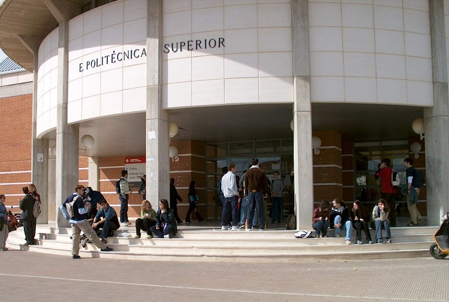
\includegraphics[width=10cm]{figs/esiiab.png}
\end{center}
\caption[Escuela Superior de Ingeniería Informática I]{Escuela Superior de Ingeniería Informática. Esto es un texto descriptivo algo más largo que puede producir un efecto feo.}
\label{fig:esiiabI}
\end{figure}



\begin{figure}[p] 
\captionsetup{width=0.8\linewidth}
\begin{center}
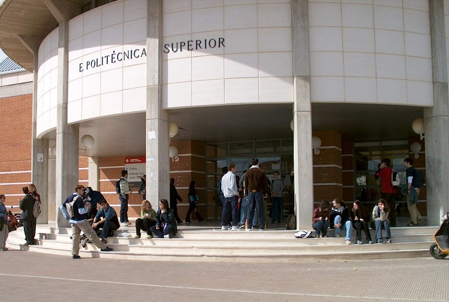
\includegraphics[width=10cm]{figs/esiiab.png}
\end{center}
\caption[Escuela Superior de Ingeniería Informática II]{Escuela Superior de Ingeniería Informática. Esto es un texto descriptivo algo más largo que puede producir un efecto feo.}
\label{fig:esiiabII}
\captionsetup{width=0.9\linewidth}
\end{figure}

Se incluye el paquete \verb+subfigure+ para la inclusión de figuras con varias imágenes o gráficas, como la que muestra la figura \ref{fig:subfiguras}.
\begin{figure}[htb]
\begin{center}
\begin{subfigure}[b]{0.4\linewidth}
\begin{center}
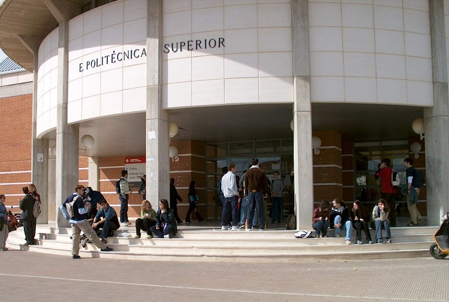
\includegraphics[width=0.9\linewidth]{figs/esiiab.png}
\caption{Fotografía de la izquierda}\label{fig:esiiabIII}
\end{center}
\end{subfigure} 
\begin{subfigure}[b]{0.4\linewidth}
\begin{center}
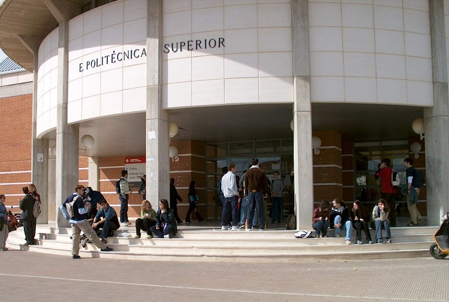
\includegraphics[width=0.9\linewidth]{figs/esiiab.png}
\caption{Fotografía de la drecha}\label{fig:esiiabIV}
\end{center}
\end{subfigure} 
\end{center}
\caption[Ejemplo de subfiguras]{Ejemplo de inclusión de subfiguras}
\label{fig:subfiguras}
\end{figure}



\section{Algoritmos y código}

Con respecto a los algoritmos (pseudocódigo) y código pueden implementarse, respectivamente, mediante el uso de los paquetes \verb+algorithmic+ y \verb+listings+. Pueden configurarse ambos entornos el archivo \verb+include\configuracion+. Por otra parte, se han definido dos entornos flotantes, denominados \verb+algorithm+ y \verb+code+ para encapsular y mostrar ambos tipos de elemento de manera uniforme.\\


El algoritmo \ref{alg:search} muestra un ejemplo de pseudocódigo. Se han añadido dos comandos, \verb+\va{variable}+ para distinguir las \va{variables}, y \verb+\fu{funcion}+ para distinguir las \fu{Funciones}. \\



\begin{algorithm}[b]
\begin{algorithmic}[1]
 	\Function{Tree-Search}{ }
 	\State \va{open} $\leftarrow$ \Call{CreateNode}{\fu{Initial-State}} \Comment{Creates the root}
	\While {\va{open} $\neq \emptyset$}
		\State \va{node} $\leftarrow$ \Call{Extract}{\va{open}}
		\If {\Call{TestGoal}{\va{node.STATE}}}
			\State \Return \Call{RecoverPath}{\va{node}} \Comment{Solution found}
		\EndIf		
				
		\State \va{successors} $\leftarrow$ \Call{Expand}{\va{node}}
		\ForAll {\va{successor} \bft{en} \va{successors}} \Comment{Processes each successor }
			\State  \Call{Insert}{\va{successor, open}}
		\EndFor	
	\EndWhile
	\State \Return failure \Comment{No solution have been found}
 	\EndFunction
\end{algorithmic}
\caption{Tree-Search exploration}
\label{alg:search}
\end{algorithm}

Por último, el listado \ref{alg:code} muestra el código del algoritmo \ref{alg:search} en \textit{Python}. El paquete \verb+listings+  contiene multitud de opciones para el manejo de distintos lenguajes y para personalización.

\begin{code}
\begin{lstlisting}

def search(initial):
	open = [initial]
	while open:
		node = open.pop()
		if testGoal(node):
			return recoverPath(node)
		successors = expand(node)
		for succesor in successors:
			open.append(succesor)
	return failure
		
\end{lstlisting}
\caption{Ejemplo de código en Python}
\label{alg:code}
\end{code}


\section{Bibliografía}

Esto es una cita \cite{RUSSELL} y esto otra \cite{AlphaZero}. La bibliografía se gestiona con bibtex y un estilo predefinido. No se han hecho modificaciones de momento.

\section{Notación matemática}

Utiliza las fuentes por defecto del tema, aunque también se pueden cambiar.


\[
J(\theta)=\frac{1}{2m}\left[ \sum_{i=1}^m\left(h_\theta(x^{(i)})-y^{(i)}\right)^2 + \lambda \sum_{j=1}^n \theta_j^2 \right], \mbox{ } \lambda >0
\]

